\documentclass[12pt,a4paper,openany]{book}
\usepackage{lmodern}
\usepackage[svgnames]{xcolor} % Required to specify font color
\usepackage{xcolor}
\definecolor{vert1}{rgb}{0.0,0.3.9,0.0}
\definecolor{bleu}{rgb}{0,0,0.5}
\definecolor{bleu3}{rgb}{1,0.2,0.2}
\definecolor{grisgris}{gray}{0.4}
\definecolor{grisclair}{HTML}{E7E7E7}
\definecolor{grisfonce}{HTML}{A5A5A5}
\definecolor{rougeUPS}{rgb}{0.6, 0.3, 0.3}

\fboxsep =0pt \parindent =0pt\parskip =12pt



\usepackage[utf8]{inputenc} 
\usepackage[T1]{fontenc}
\usepackage{wrapfig}
\usepackage[francais]{babel}
\usepackage[top=1.7cm, bottom=1.7cm, left=1.7cm, right=1.7cm]{geometry}
\usepackage{verbatim}
\usepackage[urlbordercolor={1 1 1}, linkbordercolor={1 1 1}, linkcolor=vert1, urlcolor=bleu, colorlinks=true]{hyperref}
\usepackage{tikz} %Vectoriel
\usepackage{listings}
\usepackage{fancyhdr}
\usepackage{multido}
\usepackage{amssymb}
\usepackage{float}
\usepackage[francais]{minitoc}
\usepackage[final]{pdfpages} 
\usepackage{graphicx} % Required for box manipulation

\newcommand{\titre}{Ressources humaines}
\newcommand{\subtitle}{UE d'ouverture}
\newcommand{\auteur}{Antoine de \bsc{Roquemaurel}}
\newcommand{\formation}{L3 Informatique}
\newcommand{\semestre}{6}
\newcommand{\annee}{2014}
\newcommand{\prof}{}


\newcommand{\pole}{}
\newcommand{\sigle}{drh}


\definecolor{gris1}{gray}{0.40}
\definecolor{gris2}{gray}{0.55}
\definecolor{gris3}{gray}{0.65}
\definecolor{gris4}{gray}{0.50}
\definecolor{vert}{rgb}{0,0.4,0}
\definecolor{violet}{rgb}{0.65, 0.2, 0.65}
\definecolor{bleu1}{rgb}{0,0,0.8}
\definecolor{bleu2}{rgb}{0,0.2,0.6}
\definecolor{bleu3}{rgb}{0,0.2,0.2}
\definecolor{rouge}{HTML}{F93928}


\lstdefinelanguage{algo}{%
   morekeywords={%
    %%% couleur 1
		importer, programme, glossaire, fonction, procedure, constante, type, 
	%%% IMPORT & Co.
		si, sinon, alors, fin, tantque, debut, faire, lorsque, fin lorsque, 
		declenche, declencher, enregistrement, tableau, retourne, retourner, =, pour, a,
		/=, <, >, traite,exception, 
	%%% types 
		Entier, Reel, Booleen, Caractere, Réél, Booléen, Caractère,
	%%% types 
		entree, maj, sortie,entrée,
	%%% types 
		et, ou, non,
	},
  sensitive=true,
  morecomment=[l]{--},
  morestring=[b]',
}

\lstset{language=algo,
    %%% BOUCLE, TEST & Co.
      emph={importer, programme, glossaire, fonction, procedure, constante, type},
      emphstyle=\color{bleu2},
    %%% IMPORT & Co.  
	emph={[2]
		si, sinon, alors, fin , tantque, debut, faire, lorsque, fin lorsque, 
		declencher, retourner, et, ou, non,enregistrement, retourner, retourne, 
		tableau, /=, <, =, >, traite,exception, pour, a
	},
      emphstyle=[2]\color{bleu1},
    %%% FONCTIONS NUMERIQUES
      emph={[3]Entier, Reel, Booleen, Caractere, Booléen, Réél, Caractère},
      emphstyle=[3]\color{gris1},
    %%% FONCTIONS NUMERIQUES
      emph={[4]entree, maj, sortie, entrée},	
      emphstyle=[4]\color{gris1},
}
\lstdefinelanguage{wl}{%
   morekeywords={%
    %%% couleur 1
		importer, programme, glossaire, fonction, procedure, constante, type, 
	%%% IMPORT & Co.
		si, sinon, alors, fin, TANTQUE, tantque, FIN, PROCEDURE, debut, faire, lorsque, 
		fin lorsque, declenche, declencher, enregistrement, tableau, retourne, retourner, =, 
		/=, <, >, traite,exception, 
	%%% types 
		Entier, Reel, Booleen, Caractere, Réél, Booléen, Caractère,
	%%% types 
		entree, maj, sortie,entrée,
	%%% types 
		et, ou, non,
	},
  sensitive=true,
  morecomment=[l]{//},
  morestring=[b]',
}

\lstset{language=wl,
    %%% BOUCLE, TEST & Co.
      emph={importer, programme, glossaire, fonction, procedure, constante, type},
      emphstyle=\color{bleu2},
    %%% IMPORT & Co.  
	emph={[2]
		si, sinon, alors, fin , tantque, debut, faire, lorsque, fin lorsque, 
		declencher, retourner, et, ou, non,enregistrement, retourner, retourne, 
		tableau, /=, <, =, >, traite,exception
	},
      emphstyle=[2]\color{bleu1},
    %%% FONCTIONS NUMERIQUES
      emph={[3]Entier, Reel, Booleen, Caractere, Booléen, Réél, Caractère},
      emphstyle=[3]\color{gris1},
    %%% FONCTIONS NUMERIQUES
      emph={[4]entree, maj, sortie, entrée},	
      emphstyle=[4]\color{gris1},
}
\lstdefinelanguage{css}{%
   morekeywords={%
    %%% couleur 1
		background, image, repeat, position, index, color, border, font, 
		size, url, family, style, variant, weight, letter, spacing, line, 
		height, text, decoration, align, indent, transform, shadow, 
		background, image, repeat, position, index, color, border, font, 
		size, url, family, style, variant, weight, letter, spacing, line, 
		height, text, decoration, align, indent, transform, shadow, 
		vertical, align, white, space, word, spacing,attachment, width, 
		max, min, margin, padding, clip, direction, display, overflow,
		visibility, clear, float, top, right, bottom, left, list, type, 
		collapse, side, empty, cells, table, layout, cursor, marks, page, break,
		before, after, inside, orphans, windows, azimuth, after, before, cue, 
		elevation, pause, play, during, pitch, range, richness, spek, header, 
		numeral, punctuation, rate, stress, voice, volume,
	%%% types 
		left, right, bottom, top, none, center, solid, black, blue, red, green,
	},
  sensitive=true,
  sensitive=true,
  morecomment=[s]{/*}{*/},
  morestring=[b]',
}
\lstset{language=css,
    %%% BOUCLE, TEST & Co.
      emph={
		background, image, repeat, position, index, color, border, font, 
		size, url, family, style, variant, weight, letter, spacing, line, 
		height, text, decoration, align, indent, transform, shadow, 
		background, image, repeat, position, index, color, border, font, 
		size, url, family, style, variant, weight, letter, spacing, line, 
		height, text, decoration, align, indent, transform, shadow, 
		vertical, align, white, space, word, spacing,attachment, width, 
		max, min, margin, padding, clip, direction, display, overflow,
		visibility, clear, float, top, right, bottom, left, list, type, 
		collapse, side, empty, cells, table, layout, cursor, marks, page, break,
		before, after, inside, orphans, windows, azimuth, after, before, cue, 
		elevation, pause, play, during, pitch, range, richness, spek, header, 
		numeral, punctuation, rate, stress, voice, volume,
	  },
      emphstyle=\color{bleu2},
    %%% FONCTIONS NUMERIQUES
      emph={[3]
		left, right, bottom, top,none, solid, black, blue, green,
		  },
      emphstyle=[3]\color{bleu3},
    %%% FONCTIONS NUMERIQUES
}

\lstset{language=SQL,
    %%% BOUCLE, TEST & Co.
      emph={INSERT, UPDATE, DELETE, WHERE, SET, GROUP, BY, ORDER, REFERENCES},
      emphstyle=\color{bleu2},
    %%% IMPORT & Co.  
	emph={[2]
		if, end, begin, then, for, each, else, after, of, on, to
	},
      emphstyle=[2]\color{bleu1},
    %%% FONCTIONS NUMERIQUES
      emph={[3]Entier, Reel, Booleen, Caractere, Booléen, Réél, Caractère},
      emphstyle=[3]\color{gris1},
    %%% FONCTIONS NUMERIQUES
      emph={[4]entree, maj, sortie, entrée},	
      emphstyle=[4]\color{gris1},
}
\lstdefinelanguage{ARM}{%
   morekeywords={%
   ADD, SUB, MOV, MUL, RSB,CMP, BLS, BLE, B,BHI,LDR,
   BGE, RSBLT, BGT, BEQ, BNE,BLT,BHS,STR,STRB
	},
  sensitive=true,
  morecomment=[l]{@},
  morestring=[b]',
}

\lstset{ % general style for listings 
   numbers=left 
   , literate={é}{{\'e}}1 {è}{{\`e}}1 {à}{{\`a}}1 {ê}{{\^e}}1 {É}{{\'E}}1 {ô}{{\^o}}1 {€}{{\euro}}1{°}{{$^{\circ}$}}1 {ç}{ {c}}1 {ù}{u}1
	, extendedchars=\true
   , tabsize=2 
   , frame=l
   , framerule=1.1pt
   , linewidth=520px
   , breaklines=true 
   , basicstyle=\footnotesize\ttfamily 
   , numberstyle=\tiny\ttfamily 
   , framexleftmargin=0mm 
   , xleftmargin=0mm 
   , captionpos=b 
	, keywordstyle=\color{bleu2}
	, commentstyle=\color{vert}
	, stringstyle=\color{rouge}
	, showstringspaces=false
	, extendedchars=true
	, mathescape=true
} 
%	\lstlistoflistings
%	\addcontentsline{toc}{part}{List of code examples}

\documentclass[12pt,a4paper,openany]{book}
\usepackage{lmodern}
\usepackage{xcolor}
\usepackage{xcolor}
\definecolor{vert1}{rgb}{0.0,0.3.9,0.0}
\definecolor{bleu}{rgb}{0,0,0.5}
\definecolor{bleu3}{rgb}{1,0.2,0.2}
\definecolor{grisgris}{gray}{0.4}
\definecolor{grisclair}{HTML}{E7E7E7}
\definecolor{grisfonce}{HTML}{A5A5A5}
\definecolor{rougeUPS}{rgb}{0.6, 0.3, 0.3}

\fboxsep =0pt \parindent =0pt\parskip =12pt



\usepackage[utf8]{inputenc}
\usepackage[T1]{fontenc}
\usepackage[francais]{babel}
\usepackage[top=1.7cm, bottom=1.7cm, left=1.7cm, right=1.7cm]{geometry}
\usepackage{verbatim}
\usepackage[urlbordercolor={1 1 1}, linkbordercolor={1 1 1}, linkcolor=vert1, urlcolor=bleu, colorlinks=true]{hyperref}
\usepackage{tikz} %Vectoriel
\usepackage{listings}
\usepackage{fancyhdr}
\usepackage{multido}
\usepackage{amssymb}
\usepackage{float}

\newcommand{\titre}{Complexité des algorithmes}

\newcommand{\pole}{}
\newcommand{\sigle}{complexite}

\newcommand{\semestre}{3}

\definecolor{gris1}{gray}{0.40}
\definecolor{gris2}{gray}{0.55}
\definecolor{gris3}{gray}{0.65}
\definecolor{gris4}{gray}{0.50}
\definecolor{vert}{rgb}{0,0.4,0}
\definecolor{violet}{rgb}{0.65, 0.2, 0.65}
\definecolor{bleu1}{rgb}{0,0,0.8}
\definecolor{bleu2}{rgb}{0,0.2,0.6}
\definecolor{bleu3}{rgb}{0,0.2,0.2}
\definecolor{rouge}{HTML}{F93928}


\lstdefinelanguage{algo}{%
   morekeywords={%
    %%% couleur 1
		importer, programme, glossaire, fonction, procedure, constante, type, 
	%%% IMPORT & Co.
		si, sinon, alors, fin, tantque, debut, faire, lorsque, fin lorsque, 
		declenche, declencher, enregistrement, tableau, retourne, retourner, =, pour, a,
		/=, <, >, traite,exception, 
	%%% types 
		Entier, Reel, Booleen, Caractere, Réél, Booléen, Caractère,
	%%% types 
		entree, maj, sortie,entrée,
	%%% types 
		et, ou, non,
	},
  sensitive=true,
  morecomment=[l]{--},
  morestring=[b]',
}

\lstset{language=algo,
    %%% BOUCLE, TEST & Co.
      emph={importer, programme, glossaire, fonction, procedure, constante, type},
      emphstyle=\color{bleu2},
    %%% IMPORT & Co.  
	emph={[2]
		si, sinon, alors, fin , tantque, debut, faire, lorsque, fin lorsque, 
		declencher, retourner, et, ou, non,enregistrement, retourner, retourne, 
		tableau, /=, <, =, >, traite,exception, pour, a
	},
      emphstyle=[2]\color{bleu1},
    %%% FONCTIONS NUMERIQUES
      emph={[3]Entier, Reel, Booleen, Caractere, Booléen, Réél, Caractère},
      emphstyle=[3]\color{gris1},
    %%% FONCTIONS NUMERIQUES
      emph={[4]entree, maj, sortie, entrée},	
      emphstyle=[4]\color{gris1},
}
\lstdefinelanguage{wl}{%
   morekeywords={%
    %%% couleur 1
		importer, programme, glossaire, fonction, procedure, constante, type, 
	%%% IMPORT & Co.
		si, sinon, alors, fin, TANTQUE, tantque, FIN, PROCEDURE, debut, faire, lorsque, 
		fin lorsque, declenche, declencher, enregistrement, tableau, retourne, retourner, =, 
		/=, <, >, traite,exception, 
	%%% types 
		Entier, Reel, Booleen, Caractere, Réél, Booléen, Caractère,
	%%% types 
		entree, maj, sortie,entrée,
	%%% types 
		et, ou, non,
	},
  sensitive=true,
  morecomment=[l]{//},
  morestring=[b]',
}

\lstset{language=wl,
    %%% BOUCLE, TEST & Co.
      emph={importer, programme, glossaire, fonction, procedure, constante, type},
      emphstyle=\color{bleu2},
    %%% IMPORT & Co.  
	emph={[2]
		si, sinon, alors, fin , tantque, debut, faire, lorsque, fin lorsque, 
		declencher, retourner, et, ou, non,enregistrement, retourner, retourne, 
		tableau, /=, <, =, >, traite,exception
	},
      emphstyle=[2]\color{bleu1},
    %%% FONCTIONS NUMERIQUES
      emph={[3]Entier, Reel, Booleen, Caractere, Booléen, Réél, Caractère},
      emphstyle=[3]\color{gris1},
    %%% FONCTIONS NUMERIQUES
      emph={[4]entree, maj, sortie, entrée},	
      emphstyle=[4]\color{gris1},
}
\lstdefinelanguage{css}{%
   morekeywords={%
    %%% couleur 1
		background, image, repeat, position, index, color, border, font, 
		size, url, family, style, variant, weight, letter, spacing, line, 
		height, text, decoration, align, indent, transform, shadow, 
		background, image, repeat, position, index, color, border, font, 
		size, url, family, style, variant, weight, letter, spacing, line, 
		height, text, decoration, align, indent, transform, shadow, 
		vertical, align, white, space, word, spacing,attachment, width, 
		max, min, margin, padding, clip, direction, display, overflow,
		visibility, clear, float, top, right, bottom, left, list, type, 
		collapse, side, empty, cells, table, layout, cursor, marks, page, break,
		before, after, inside, orphans, windows, azimuth, after, before, cue, 
		elevation, pause, play, during, pitch, range, richness, spek, header, 
		numeral, punctuation, rate, stress, voice, volume,
	%%% types 
		left, right, bottom, top, none, center, solid, black, blue, red, green,
	},
  sensitive=true,
  sensitive=true,
  morecomment=[s]{/*}{*/},
  morestring=[b]',
}
\lstset{language=css,
    %%% BOUCLE, TEST & Co.
      emph={
		background, image, repeat, position, index, color, border, font, 
		size, url, family, style, variant, weight, letter, spacing, line, 
		height, text, decoration, align, indent, transform, shadow, 
		background, image, repeat, position, index, color, border, font, 
		size, url, family, style, variant, weight, letter, spacing, line, 
		height, text, decoration, align, indent, transform, shadow, 
		vertical, align, white, space, word, spacing,attachment, width, 
		max, min, margin, padding, clip, direction, display, overflow,
		visibility, clear, float, top, right, bottom, left, list, type, 
		collapse, side, empty, cells, table, layout, cursor, marks, page, break,
		before, after, inside, orphans, windows, azimuth, after, before, cue, 
		elevation, pause, play, during, pitch, range, richness, spek, header, 
		numeral, punctuation, rate, stress, voice, volume,
	  },
      emphstyle=\color{bleu2},
    %%% FONCTIONS NUMERIQUES
      emph={[3]
		left, right, bottom, top,none, solid, black, blue, green,
		  },
      emphstyle=[3]\color{bleu3},
    %%% FONCTIONS NUMERIQUES
}

\lstset{language=SQL,
    %%% BOUCLE, TEST & Co.
      emph={INSERT, UPDATE, DELETE, WHERE, SET, GROUP, BY, ORDER, REFERENCES},
      emphstyle=\color{bleu2},
    %%% IMPORT & Co.  
	emph={[2]
		if, end, begin, then, for, each, else, after, of, on, to
	},
      emphstyle=[2]\color{bleu1},
    %%% FONCTIONS NUMERIQUES
      emph={[3]Entier, Reel, Booleen, Caractere, Booléen, Réél, Caractère},
      emphstyle=[3]\color{gris1},
    %%% FONCTIONS NUMERIQUES
      emph={[4]entree, maj, sortie, entrée},	
      emphstyle=[4]\color{gris1},
}
\lstdefinelanguage{ARM}{%
   morekeywords={%
   ADD, SUB, MOV, MUL, RSB,CMP, BLS, BLE, B,BHI,LDR,
   BGE, RSBLT, BGT, BEQ, BNE,BLT,BHS,STR,STRB
	},
  sensitive=true,
  morecomment=[l]{@},
  morestring=[b]',
}

\lstset{ % general style for listings 
   numbers=left 
   , literate={é}{{\'e}}1 {è}{{\`e}}1 {à}{{\`a}}1 {ê}{{\^e}}1 {É}{{\'E}}1 {ô}{{\^o}}1 {€}{{\euro}}1{°}{{$^{\circ}$}}1 {ç}{ {c}}1 {ù}{u}1
	, extendedchars=\true
   , tabsize=2 
   , frame=l
   , framerule=1.1pt
   , linewidth=520px
   , breaklines=true 
   , basicstyle=\footnotesize\ttfamily 
   , numberstyle=\tiny\ttfamily 
   , framexleftmargin=0mm 
   , xleftmargin=0mm 
   , captionpos=b 
	, keywordstyle=\color{bleu2}
	, commentstyle=\color{vert}
	, stringstyle=\color{rouge}
	, showstringspaces=false
	, extendedchars=true
	, mathescape=true
} 
%	\lstlistoflistings
%	\addcontentsline{toc}{part}{List of code examples}
 %prise en charge du langage C 
\date{\today}

\makeindex
\lfoot{Université Toulouse III -- Paul Sabatier}
\rfoot{\sigle\semestre}
%\rfoot{}
\cfoot{}
\makeglossary
\makeatletter
\def\clap#1{\hbox to 0pt{\hss #1\hss}}%
\def\ligne#1{%
\hbox to \hsize{%
\vbox{\centering #1}}}%
\def\haut#1#2#3{%
\hbox to \hsize{%
\rlap{\vtop{\raggedright #1}}%
\hss
\clap{\vtop{\centering #2}}%
\hss
\llap{\vtop{\raggedleft #3}}}}%
\def\bas#1#2#3{%
\hbox to \hsize{%
\rlap{\vbox{\raggedright #1}}%
\hss \clap{\vbox{\centering #2}}%
\hss
\llap{\vbox{\raggedleft #3}}}}%
\def\maketitle{%
\thispagestyle{empty}\vbox to \vsize{%
\haut{}{\@blurb}{}

\vfill
\vspace{1cm}
\begin{flushleft}
\usefont{OT1}{ptm}{m}{n}
\huge \@title
\end{flushleft}
\par
\hrule height 4pt
\par
\begin{flushright}
\usefont{OT1}{phv}{m}{n}
\Large \@author
\par
\end{flushright}
\vspace{1cm}
\vfill
\vfill
\bas{}{\@location, le \@date}{}
}%
\cleardoublepage
}
\def\date#1{\def\@date{#1}}
\def\author#1{\def\@author{#1}}
\def\title#1{\def\@title{#1}}
\def\location#1{\def\@location{#1}}
\def\blurb#1{\def\@blurb{#1}}
\date{\today}
\author{}
\title{}
\location{Amiens}\blurb{}
\makeatother
\title{\titre}
\author{Semestre \semestre}

\location{Toulouse}
\blurb{%
Université Toulouse III -- Paul sabatier\\
L2 Informatique\\
}%



%\title{Cours \\ \titre}
%\date{\today\\ Semestre \semestre}

%\lhead{Cours: \titre}
%\chead{}
%\rhead{\thepage}

%\lfoot{Université Paul Sabatier Toulouse III}
%\cfoot{\thepage}
%\rfoot{\sigle\semestre}

\pagestyle{fancy}
\renewcommand{\chaptermark}[1]{\markboth{\bsc{\chaptername~\thechapter{} :} #1}{}}
\renewcommand{\sectionmark}[1]{\markright{\thesection{ #1}}}
\renewcommand{\headrulewidth}{0.3pt}
\renewcommand{\footrulewidth}{0.3pt}

\fancyhf{}
\fancyhead[LE]{\leftmark}
\fancyhead[RO]{\rightmark}
\fancyfoot[LE,RO]{--~\thepage~--}
\fancyfoot[LO]{\titre{}~~---~~\sigle{}\semestre{}}
\fancyfoot[RE]{Antoine de \bsc{Roquemaurel}}

%% Cas des premières pages de chapitre
\fancypagestyle{plain}{%
	\fancyhf{}%
	\fancyfoot[L]{\titre{}~~---~~\sigle{}\semestre{}}
	\fancyfoot[R]{--~\thepage~--}
	\renewcommand{\headrulewidth}{0pt}
	\renewcommand{\footrulewidth}{0.3pt}
}
\makeatletter
\renewcommand*{\lstlistlistingname}{Liste des codes sources}
\renewcommand\listoffigures{%
    \chapter{\listfigurename}%
      \@mkboth{\MakeUppercase\listfigurename}%
              {\MakeUppercase\listfigurename}%
       \@starttoc{lof}%
    }
    \renewcommand\listoftables{%
    \chapter{\listtablename}%
    \@mkboth{\MakeUppercase{\listtablename}}%
            {\MakeUppercase{\listtablename}}%
    \@starttoc{lot}
    }

    \renewcommand\lstlistoflistings{%
    \begingroup
    \chapter{\lstlistlistingname}%
    \parskip\z@\parindent\z@\parfillskip \z@ \@plus 1fil%
    \@starttoc{lol}%
    \endgroup
    }
	\makeatother

\newcommand{\remarque}[1]{
	\begin{center}
	\medskip
	\colorbox{remarque}{
		\begin{minipage}{0.85\textwidth}\medskip
\includegraphics[height=10px]{images/remarque.png} #1 \medskip\end{minipage}
	}
	\medskip
	\end{center}
}

\newcounter{exemples}

\newenvironment{exemple}[1]{
   \vspace{-2mm}

\refstepcounter{exemples}
   \begin{center}
	\medskip
      \begin{minipage}{0.9\linewidth}
}{%
~
      \end{minipage}
   \end{center}~
   \vspace{-2mm}
}%

\newcommand{\captionExemple}[1]{
	\begin{center}{\bsc{Exemple} \thechapter.\arabic{exemples}~--~}#1\end{center}
}

\DeclareTextFontCommand{\policeGlossaire}{\fontfamily{lmss}\selectfont}
\DeclareTextFontCommand{\policePackage}{\fontfamily{phv}\selectfont}
\DeclareTextFontCommand{\policeTitre}{\fontfamily{ptm}\selectfont}
\newcommand{\policeCode}[1]{\texttt{#1}}

\newcommand{\sectionfont}{%
	\fontencoding{\encodingdefault}%
	\fontfamily{pag}%
	\fontseries{bc}%
	\fontshape{n}%
	\selectfont
}

% numéro du chapitre
\DeclareFixedFont{\chapnumfont}{T1}{phv}{b}{n}{80pt}
% pour le mot « Chapitre »
\DeclareFixedFont{\chapchapfont}{T1}{phv}{b}{n}{16pt}
% pour le titre
\DeclareFixedFont{\chaptitfont}{T1}{phv}{b}{n}{24.88pt}


\makeatletter
\def\thickhrulefill{\leavevmode \leaders \hrule height 1ex \hfill \kern \z@}
%% \chapter
\def\@makechapterhead#1{%
  \reset@font
  \parindent \z@
  \vspace*{10\p@}%
  \hbox{%
    \vbox{%
      \advance\hsize by -2cm
      \hrule height 0.4pt depth 0pt width \hsize
      \par
      \vskip 6pt%
      \hspace{20pt}%
      \parbox{420pt}{%
        \LARGE \bfseries #1
		}%
      \par
      \vskip 6pt%
      \hspace{20pt}%
      \hrule height 0.4pt depth 0pt width \hsize
	  \vspace{-30pt}
      }%
    \vbox{%
      \hsize=1.5cm%
      \begin{tabular}{c}
        \scshape \large \strut \@chapapp{} \\
        \colorbox{black}{\vbox{\hbox{\vbox to 1mm{}}\hbox{
			\color{white} \LARGE \bfseries \hspace{1mm}\thechapter\hspace{1mm}
		}\hbox{\vbox to 2cm{}}}}%
      \end{tabular}%
      }%
    }%
  \vskip 20\p@
}
%% \chapter*
\def\@makeschapterhead#1{%
  \reset@font
  \parindent \z@
  \vspace*{10\p@}%
  \hbox{%
    \vbox{%
      \advance\hsize by -0cm
      \hrule height 0.4pt depth 0pt width \hsize
      \par
      \vskip 6pt%
      \hspace{20pt}%
      \parbox{420pt}{%
        \LARGE \bfseries #1
		}%
      \par
      \vskip 6pt%
      \hspace{20pt}%
      \hrule height 0.4pt depth 0pt width \hsize
      }%
    }%
  \vskip 20\p@

}

\newlength{\sectiontitleindent}
\newlength{\subsectiontitleindent}
\newlength{\subsubsectiontitleindent}
\setlength{\sectiontitleindent}{-1cm}
\setlength{\subsectiontitleindent}{-.5cm}
\setlength{\subsubsectiontitleindent}{-.25cm}

\renewcommand{\section}{%
	\@startsection%
	{section}%
	{1}%
	{\sectiontitleindent}%
	{-3.5ex plus -1ex minus -.2ex}%
	{2.3ex plus.2ex}%
	{\sectionfont\Large}
}
\renewcommand{\subsection}{%
	\@startsection%
	{subsection}%
	{2}%
	{\subsectiontitleindent}%
	{-3.5ex plus -1ex minus -.2ex}%
	{2.3ex plus.2ex}%
	{\sectionfont\large}
}

\renewcommand{\subsubsection}{%
	\@startsection%
	{subsubsection}%
	{3}%
	{\subsubsectiontitleindent}%
	{-3.5ex plus -1ex minus -.2ex}%
	{2.3ex plus.2ex}%
	{\sectionfont\normalsize}
}

\makeatother



\newcommand{\pfp}{\texttt{pfp}}

\newcommand{\ifp}{\texttt{if}}
\newcommand{\moy}{\textrm{moy}}
\newcommand{\prob}{\textrm{prob}}
\newcommand{\elsep}{\texttt{else}}

\makeatother

\begin{document}
	\setcounter{tocdepth}{1}
	\setcounter{secnumdepth}{3}
	\maketitle
	\tableofcontents
	\chapter{Introduction}
		\section{Complexité}
		On cherche à estimer le temps de calcul d'un algorithme A en fonction d'un paramètre n. Pour avoir une mesure indépendante de la machine, on identifie
		le temps de calcul avec le nombre d'instructions exécutées. 
		
		\exemple{Le paramètre n pourrait être la taille d'un tableau, par exemple.}

		Soit $D_i$ l'ensemble des données possibles telle que $n=i$. Pour $d \in D_i$ on notera $T(A,d)$ le nombre d'instructions exécutée pendant l'exécution de
		$A(d)$.\\
		On notera $\prob(d|i)$ la probabilité que les données soit $d$ étant donné qu'elles sont de taille $i$.

		\subsection{La complexité temporelle maximale} 
		La complexité temporelle maximale\footnote{Complexité dans le pire des cas} d'un algorithme A :
		$$T_{\max}(i) = \max_{d\in D_i}\{T(A,d)\}$$
		\subsection{La complexité temporelle moyenne}
		La complexité temporelle moyenne\footnote{Complexité dans le cas moyen} d'un algorithme A :
		$$T_{\moy} = \sum_{d \in D_i} \prob(d|i) \times T(A,d)$$
		\remarque{Pour pouvoir calculer $T_\moy$, il faut connaître la distribution des données, ce qui n'est pas toujours évident (par exemple en traitement d'image)}
		\subsection{La complexité temporelle minimale}
		La complexité temporelle minimale\footnote{Complexité dans le meilleur des cas} d'un algorithme A :
		$$T_{\min}(i) = \min_{d\in D_i}\{T(A,d)\}$$ 
		\remarque{Peu utilisé, sauf pour prouver qu'un algorithme est mauvais. Si la complexité temporelle minimale est 
			mauvaise même dans le meilleur des cas, alors l'algorithme n'est pas bon.}

%			\remarque{$T_{\max}$ et $T_{\min}$ nous fournissent des bornes supérieures et inférieures.}

		\subsection{Compairaison de complexités en fonction de la machine}
		\begin{tabular}{| c | p{7cm} | p{7cm}|} 
			\hline
			\textbf{Complexité}& \multicolumn{2}{|c|}{\textbf{Nombre d'instructions pouvant executer la machine}}\\
			\hline
			 & $1\;000\;000$ & $1\;000\;000\;000\;000$\\
			\hline
			$n$ & $1\;000\;000$&$1\;000\;000\;000\;000$\\
			\hline
			$n \log_2 n$ &$64\;000$&$32\;000\;000\;000$\\
			\hline
			$n^2$ & $1\;000$&$1\;000\;000$\\
			\hline
			$n^3$ &$100$&$10\;000$\\
			\hline
			$2^n$ &$20$&$40$\\
			\hline
		\end{tabular}
		\section{Complexité asymptotique}
		Pour comparer des algorithmes, on ne s'intéresse qu'à leur comportements pour n grand. On cherche une mesure de complexité qui soit indépendante du langage de programmation et de la vitesse de la machine. \\ 
	$\Rightarrow$		On ne doit pas perdre en compte des facteurs constants.  \\
	$\Rightarrow$	Ordre de grandeur

	\subsection{La complexité asymptotique}
	La complexité asymptotique\footnote{Que ce soit maximale, moyenne ou minimale} est l'ordre de grandeur de sa limite lorsque $n \rightarrow \infty$

	\subsection{Notation} Soient $T$, $f$ des fonctions positives ou nulles. Rotations de grandeur de fonction asymptotiques.
	\paragraph{Grand O} $T = O(f)$ si $\exists c \in \mathbb{R}^{>0}$ et $n_0 \in \mathbb{N}$ tels que $\forall n \geq n_0$, $T(n) \leq cf(n)$.

	\paragraph{Grand Oméga} $T = \Omega(f)$ si $\exists c \in \mathbb{R}^{>0}$ et $n_0 \in \mathbb{N}$ tels que $i\forall n \geq n_0$, $T(n) \geq cf(n)$
	\paragraph{Petit O} $T = o(f)$ si $\frac{T(n)}{f(n)} \rightarrow O$ lorsque $n \rightarrow \infty$. 
	\remarque{T est négligeable devant f}

	\exemple{
	\begin{enumerate}
		\item $2n^2 + 5n + 10 = O(n^2)$\\
		Dans la définition $n_0 = 5$,$c=4$ : \\
		$\forall n \geq 5,\ 2n^2+5n+10 \leq 4n^2$
	\item $2n^2 + 5n + 10 = \Omega(n^2)$\\
		Dans la définition, $n_0 = 1$, $c = 2$\\
		$\forall n \geq 1,\ 2n^2 + 5n + 10 \geq 2n^2 \cdots$\\
		Donc $2n^2+5n+10 = \Theta (n^2)$
	\item $\frac{1}{5} + n = O(n\log_2 n)\ (n_0 = 2,\ c=2)$
	\item $\frac{1}{5} n \log_2 n + n = \Omega(n \log n)\ (n_0=1,c=\frac{1}{5})$
	\item $\forall k \geq 0$, $n^k = O(n^{k+1})$ mais $n^k \neq \Omega(n^{k+1})$
	\item $\forall a,b >1, \log_a n = \Theta (\log_b n)$ car $\log_a n = \frac{\log_b n}{\log_b a}$ et $\log_b a$ est une constante. $\Rightarrow$ On a pas besoin de préciser la base de logarithme dnas une complexité asymptotique
	\item $2n^2 + 5n + 10 = 2n^2 + 0(n^2)$
	\item Pour toute constante $c>0$, $C = \Theta(1)$
	\item $2^n = o(3^n)$
	\end{enumerate}
	}
	\remarque{\begin{enumerate}
		\item O et $\Omega$ sont des pré-ordres\footnote{Relations reflexives et transitives} :\\ $f = O(f)$ et $f = O(g)$ et $g = O(h)) \Rightarrow f = O(h)$
		\item $\Theta$ est une relation d'équivalence\footnote{relation reflexives, symétrique et transitive} : 
			$f = \Theta(g) \Leftrightarrow g = \Theta (f)$
	\end{enumerate}
	}
	\paragraph{Proposition}
	$$\textrm{Si } \lim_{n \rightarrow \infty} \frac{f(n)}{g(n)} = a > 0 \textrm{ Alors }f = \Theta (g)$$
	\remarque{La réciproque est fausse}

	\paragraph{Notation} $$f \sim g \Rightarrow \lim_{n\rightarrow \infty} \frac{f(n)}{g(n)} = 1$$
	\exemple{$(3n+1)^3 \sim 27n^3$}
	\section{Exemple de complexités d'algorithmes}
	\subsection{Le tri à bulles}
	\begin{eqnarray*}
		T_{\min} (n) &=& \Theta (n) \textrm{ Si le tableau est est déjà trié}\\
		T_{\max}(n) &=& \Theta(n^2) \textrm{ Si le tableau est trié en ordre décroissant}\\
		T_{\moy}(n) &=& T_{\max}(n) = \Theta(n^2)\\
	\end{eqnarray*}
	\subsection{Tri par fusion}
	\begin{eqnarray*}
		T_{\min}(n) = T_{\max}(n) = T_{\moy}(n) = \Theta (n\log n)
	\end{eqnarray*}
	\subsection{Tri rapide}
	\begin{eqnarray*}
		T_{\min}(n) = T_{\moy}(n) &=& \Theta (n \log n)\\
		T_{\max}(n) &=& \Theta(n^2)
	\end{eqnarray*}
	\chapter{Complexité des boucles}
	\chapter{Complexité d'algorithmes définis par réccurence}
	\chapter{Structure de données et complexité}
	
	\appendix
	\chapter{Exercices}
	\section{TD 1}
\end{document}



\newcommand{\remarque}[1]{
	\begin{center}
	\medskip
	\colorbox{remarque}{
		\begin{minipage}{0.85\textwidth}\medskip
\includegraphics[height=10px]{images/remarque.png} #1 \medskip\end{minipage}
	}
	\medskip
	\end{center}
}

\newcounter{exemples}

\newenvironment{exemple}[1]{
   \vspace{-2mm}

\refstepcounter{exemples}
   \begin{center}
	\medskip
      \begin{minipage}{0.9\linewidth}
}{%
~
      \end{minipage}
   \end{center}~
   \vspace{-2mm}
}%

\newcommand{\captionExemple}[1]{
	\begin{center}{\bsc{Exemple} \thechapter.\arabic{exemples}~--~}#1\end{center}
}

\DeclareTextFontCommand{\policeGlossaire}{\fontfamily{lmss}\selectfont}
\DeclareTextFontCommand{\policePackage}{\fontfamily{phv}\selectfont}
\DeclareTextFontCommand{\policeTitre}{\fontfamily{ptm}\selectfont}
\newcommand{\policeCode}[1]{\texttt{#1}}

\newcommand{\sectionfont}{%
	\fontencoding{\encodingdefault}%
	\fontfamily{pag}%
	\fontseries{bc}%
	\fontshape{n}%
	\selectfont
}

% numéro du chapitre
\DeclareFixedFont{\chapnumfont}{T1}{phv}{b}{n}{80pt}
% pour le mot « Chapitre »
\DeclareFixedFont{\chapchapfont}{T1}{phv}{b}{n}{16pt}
% pour le titre
\DeclareFixedFont{\chaptitfont}{T1}{phv}{b}{n}{24.88pt}


\makeatletter
\def\thickhrulefill{\leavevmode \leaders \hrule height 1ex \hfill \kern \z@}
%% \chapter
\def\@makechapterhead#1{%
  \reset@font
  \parindent \z@
  \vspace*{10\p@}%
  \hbox{%
    \vbox{%
      \advance\hsize by -2cm
      \hrule height 0.4pt depth 0pt width \hsize
      \par
      \vskip 6pt%
      \hspace{20pt}%
      \parbox{420pt}{%
        \LARGE \bfseries #1
		}%
      \par
      \vskip 6pt%
      \hspace{20pt}%
      \hrule height 0.4pt depth 0pt width \hsize
	  \vspace{-30pt}
      }%
    \vbox{%
      \hsize=1.5cm%
      \begin{tabular}{c}
        \scshape \large \strut \@chapapp{} \\
        \colorbox{black}{\vbox{\hbox{\vbox to 1mm{}}\hbox{
			\color{white} \LARGE \bfseries \hspace{1mm}\thechapter\hspace{1mm}
		}\hbox{\vbox to 2cm{}}}}%
      \end{tabular}%
      }%
    }%
  \vskip 20\p@
}
%% \chapter*
\def\@makeschapterhead#1{%
  \reset@font
  \parindent \z@
  \vspace*{10\p@}%
  \hbox{%
    \vbox{%
      \advance\hsize by -0cm
      \hrule height 0.4pt depth 0pt width \hsize
      \par
      \vskip 6pt%
      \hspace{20pt}%
      \parbox{420pt}{%
        \LARGE \bfseries #1
		}%
      \par
      \vskip 6pt%
      \hspace{20pt}%
      \hrule height 0.4pt depth 0pt width \hsize
      }%
    }%
  \vskip 20\p@

}

\newlength{\sectiontitleindent}
\newlength{\subsectiontitleindent}
\newlength{\subsubsectiontitleindent}
\setlength{\sectiontitleindent}{-1cm}
\setlength{\subsectiontitleindent}{-.5cm}
\setlength{\subsubsectiontitleindent}{-.25cm}

\renewcommand{\section}{%
	\@startsection%
	{section}%
	{1}%
	{\sectiontitleindent}%
	{-3.5ex plus -1ex minus -.2ex}%
	{2.3ex plus.2ex}%
	{\sectionfont\Large}
}
\renewcommand{\subsection}{%
	\@startsection%
	{subsection}%
	{2}%
	{\subsectiontitleindent}%
	{-3.5ex plus -1ex minus -.2ex}%
	{2.3ex plus.2ex}%
	{\sectionfont\large}
}

\renewcommand{\subsubsection}{%
	\@startsection%
	{subsubsection}%
	{3}%
	{\subsubsectiontitleindent}%
	{-3.5ex plus -1ex minus -.2ex}%
	{2.3ex plus.2ex}%
	{\sectionfont\normalsize}
}

\makeatother



\newcommand{\pfp}{\texttt{pfp}}

\newcommand{\ifp}{\texttt{if}}
\newcommand{\elsep}{\texttt{else}}

\usepackage{ifthen}

\newsavebox{\fmbox}
\newenvironment{fmpage}[1]
     {\begin{lrbox}{\fmbox}\begin{minipage}{#1}}
	  {\end{minipage}\end{lrbox}\fbox{\usebox{\fmbox}}}


\makeatletter

\title{Projet Agile --- \bsc{SCRUM}}

\def\top#1{\def\@top{#1}}

\def\sousTitre#1{\def\@sousTitre{#1}}
\sousTitre{Rubidium}

\def\location#1{\def\@location{#1}}
\location{Toulouse}

\date{\today}

%% Entete (Université..)  
\def\clap#1{
	\hbox to 0pt{\hss #1\hss}
}%
\def\ligne#1{%
	\hbox to \hsize{%
		\vbox{\centering #1}
	}
}%

% définition du haut de la couverture %
\def\haut#1#2#3{%
	\hbox to \hsize{%
		\rlap{
			\vtop{\raggedright #1}
		}%
		\hss
		\clap{	
			\vtop{\centering #2}
		}%
		\hss
		\llap{
			\vtop{\raggedleft #3}
		}
	}
}%

% Définition du bas de la couverture %
\def\bas#1#2#3{%
	\hbox to \hsize{%
	\hss \clap{\vbox{
	\centering \hspace{1.7cm}\newline
		\newline \newline \newline	\newline \newline \newline	\newline \newline \newline	\newline \newline \newline	\newline \newline \newline	\newline \newline \newline\newline #2 }
		}%
		\hss
	}
}%

% Zou, on peut construire la page de garde 
\def\maketitle{%
	\thispagestyle{empty}\vbox to \vsize{%
		\vspace{-25px}
		\vspace{5px}
		\haut{}{\@top}{}
		\vfill
		\begin{flushleft}
			David \bsc{Bernard}\\
			Mathias \bsc{Faure}\\
			Antoine \bsc{Incorvaia}\\
			Lucas \bsc{Le gouic}\\
			Antoine de \bsc{Roquemaurel}\\
			Clément \bsc{Vannier}\\
		\end{flushleft}

		\begin{flushright}
			\vspace{-3cm}
			\begin{tabular}{r@{~}l}
				Pour M. \bsc{Fernandez} 
			\end{tabular}
		\end{flushright}
		\vfill
		\vspace{1cm}
		\begin{flushleft}
			\policeTitre{\huge \@title}
		\end{flushleft}

		\par
		\hrule height 4pt
		\par

		\begin{flushright}
			\policeTitre{\Large \@sousTitre}
			\par
		\end{flushright}
		\vspace{3.2cm}
		\bas{}{ \@location, le \@date}{}
		\vspace{5px}
		\vspace{-15px}
	}%
	\cleardoublepage
}

\makeatother

\top{%
	Université Paul Sabatier -- Toulouse III\\
	IUT A - Toulouse Rangueil\\
	%\textbf{Projet tuteuré \#20}\\[1em]
}%

\makeatletter

\makeatother
\pagestyle{fancy}

\makeatother
\includeonly {
eco,
drh,
entreprisesCotes
}
\begin{document}
	\thispagestyle{empty} % Removes page numbers
	\titleBC 
	\dominitoc
	\setcounter{tocdepth}{1}
	\setcounter{secnumdepth}{3}
	\setcounter{minitocdepth}{1}
	\tableofcontents
	\part{Économie}
		\chapter{Qu'est-ce que l'économie}
	\section{Introduction}
	\subsection{Définitions préalables}
	\subsubsection{Economie}
		<< règles de conduites des affaires domestiques >>, élargit à la nation
		\subsection{Science économique}
		Se définit par un objet d'étude et une méthodologie.

	On définit le besoin économique comme un manque qui peut être satisfait par l'acquisition ou la consommation de besoin et service sachant qu'ils
	sont en produit en quantité limité.

	Comme les ressources en matière première sont rares, il est impossible de produire tous les biens nécessaire à la satisfaction des besoins
	nécessaire, ainsi la science économique va essayer de régler ce problème. Pour appréhender la réalité la science économique va reposer sur des
	modélisations.

	La sciences économique est une approche positive et non une approche normative.

	\subsubsection{Macro-économie}
	Étude de l'économie en général, elle porte l'intérêt sur des variables (agrégats), meusrées par la comptabilité nationale. 
	\begin{exemple}
		Augmentation du niveau général des prix dans l'économie	
	\end{exemple}
	\subsubsection{Micro-économie}
	Analyse des comportements individuels des agents économique dans le but de comprendre leur processus de décision
	\subsubsection{Méso-économie}
	Analyse des groupes (une branches, une filières, un secteur) qui détiennent un pouvoir suffisant pour influencer l'économie nationale.

	\subsection{Questions récurrentes aujourd'hui}
	\begin{itemize}
		\item Quel est le niveau de la croissance ? Comment est-elle répartie ? 
		\item La crise pourra-t-elle est enrayée ? 
		\item La mondialisation est-elle responsable de tous les maux ? 
	\end{itemize}

	Un bref retour sur << le >> contexte en France:
	\begin{itemize}
		\item Phénomène de désindustrialisation : Certains facteur traduisent l'affaiblissement de la France pare qu'il y  eu une industrialisation du
		\item Faiblesse d'entreprise de taille intermédiaire et donc un manque de PME exportatrice.  bas de gamme.
		\item Le taux de chômage
		\item La responsabilité sociétale des entreprises
		\item Un nouveau modèle économique : l'économie du partage  production, distribution, échange, consommation, \ldots
	\end{itemize}

	\subsection{Les types d'entreprises}
	\begin{itemize}
		\item Micro entreprise : moins de 10 personnes, un CA annuel ou un total de bilan n'excédant pas 2 millions d'euros.
		\item PME : moins de 250 personnes, un CA annuel n'excédant par 50 millions d'euros ou un total de bilan n'excédant pas 43 millions.
		\item Entreprise de traille intermédiaire : moins de 5000 personnes
		\item Grandes entreprises : plus de 5000 salariés
	\end{itemize}

	En 2012 environ 3.5 millions d'entreprise en France, 67\% des entreprises française n'ont aucun salarié, 94\% ont de 0 à 9 salariés, et 99\% ont de
	0 à 49 salariés.

	\section{L'activité économique et ses agents}
	\begin{definition}
		Un agent économique est un individu ou groupement d'individus qui s'organise et prend des décisions économiques pour satisfaire ses besoins et
		lutter contre la rareté.
	\end{definition}

	On distingue 6 catégories d'agents économiques de par leur fonction économique principale : 
	\begin{description}
		\item[Les entreprises]Production de biens et services marchants et distribution de la richesse grâce à la combinaison de facteurs de
			production tel que le travail est la capital
		\item[Les ménages] Consommation de bien et services rendue possible grâce aux revenus que le ménage perçois, revenu qui est obtenir pour
			l'essentiel en échange de leur travail mais également de revenus secondaires.\\~
			$$revenuPrimaire + revenuSecondaires - Impots = RevenuDisponibleBrut$$

			\begin{remarque}
				\begin{itemize}
					\item La consommation des ménages est un des agrégats les plus stable de l'économie.
					\item La consommation ne dépend pas toujours du niveau de revenus.
					\item La partie non consommée par les revenus est appelé l'épargne
				\end{itemize}
			\end{remarque}
		\item[Les institutions financières] Gestion des produits financiers, opérations de crédit, gestion des moyens de paiement.\\
			La banque centrale auquel les banques se refinance, qui émet de la monnaie et qui limite la création monétaire plus qu'elle va contrôler le
			montant des crédits par exemple.
		\item[Le secteur public] Fournitures des services non marchands, redistribution, régulation. Il se compose des administrations publiques,
			l'état, les collectivités locale, la sécurité sociale, \ldots 
		\item[L'extérieur] Opérations entre entités résidentes et non résidentes.
	\end{description}

	\section{Le circuit économique}
	Le circuit économique permet de représenter les relations qui existent entre les agents économiques. Les relations s'effectue par des flux réels et
	des flux monétaires.

	\subsection{La comptabilité nationale et la mesure de l'activité}
	Les agents économiques regroupés en catégories d'acteurs sont rassemblés dans un cadre: la comptabilité nationale.

	La comptabilité nationale est une représentation chiffrée de l'économie nationale qui sert à faire des simulations sur la croissance économique et
	donc des prévisions sur le budget de 'état.

	Elle produit: 
	\begin{itemize}
		\item Le tableau économique d'ensemble (TEE)
		\item Le tableau des entrées/sorties (TES)
	\end{itemize}

	\part{Ressources humaines}
		\chapter*{Introduction}
	Dans une entreprise, il y a 6 ressources : 
	\begin{itemize}
		\item Humaines
		\item Recherche et développement
		\item Production 
		\item Commerciale
		\item Finances 
		\item Information
	\end{itemize}

	Chacune de ces ressources à un directeur\footnote{Directeur commercial, Directeur
	Ressources humains, Directeur financier, \ldots}, ici nous aborderons principalement
	les ressources humaines.
	
	\chapter{Réussir un entretien}

	En arrivant dans une entreprise on demande un projet, à distinguer avec un
	objectif\footnote{Exemple d'objectif, devenir ingénieur développement}, un projet est
	lié à la motivation : << qu'est ce que j'ai envie de faire ? >>, afin d'être pris au
	sérieux il faut donc dire ce qu'on veut faire, ce qu'on va apporter à
	l'entreprise.

	Afin d'effectuer une bonne carrière, deux compétences sont très importantes: 
	\begin{description}
		\item[Communication] Clients, Hiérarchie, \ldots
		\item[Négociation] Salaires, postes, clients, \ldots
		\item[Management] Gérer une équipe, motiver les gens, les faire collaborer, donner envie de travailler,\ldots
	\end{description}

	Évaluation des compétences : 
	\begin{description}
		\item[Savoir] Diplôme
		\item[Savoir faire] Expérience
		\item[Savoir être] Attitudes générale
	\end{description}

	\chapter{Les ressources humaines}
	Les ressources humaines sont là pour gérer le personnel, elles doivent aider à faire avancer le personnel.

	Chaque personne de l'entreprise à du potentiel : Avoir des compétences mais aussi de la motivation. 

	Les ressources humaines sont là pour que le plus de personnes ai le maximum de résultats, avec une bonne rh, personne ne doit se retrouver en bas à
	gauche.

	\begin{figure}[H]
		\centering
		\includegraphics[width=5cm]{figure1.eps}
	\end{figure}
	Une entreprise doit avoir beaucoup d'espoirs et pilliers, éviter trop d'étoiles, pour éviter les conflits.

	\section{Objectifs d'un DRH}
	\begin{description}
		\item[Abaisser les effectifs] préférer enrichir les postes des utilisateurs
		\item[Abaisser la masse salariale] Réduire les échelons, utiliser des logiciels de gestion, \ldots
		\item[Multiplier les compétences] 
	\end{description}

	\section{Finalité de la RH}
	\subsection{Recruter}
	Travailler avec la hiérarchie pour décrire le post, trouver les compétences nécessaire et vont chercher les profils nécessaires.
	\begin{remarque}
		Pour une candidature spontanée, ils est préférable de contacter le directeur du service plutôt que la RH: les RH auront une approche qui
		concerne plus la gestion de l'entreprise(pyramides des ages, diplômes, experience, \ldots) alors que le service regardera les compétences.
	\end{remarque}

	\subsection{Former}
	La formation interne à l'entreprise : faire en sorte que l'entreprise ai les compétences nécessaires au bon moment.

	\subsection{Gérer}
	Gérer les effectifs\footnote{savoir combien il y a de personnes qui travaillent à un instant T}, les congés, les RTT, les crédits formations.
	
	\subsection{Administration}
	Suivis administratif des gens : faire évoluer leur état civil, coefficient en fonction du poste, \ldots

	\subsection{Négocier}
	Obligation de négocier tous le ans avec les syndicats.(Sans obligation d'aboutissement) 

	\subsection{Organiser}
	Organisation du travail optimal.

	\subsection{Communication}
	Deux types : externe et interne. 

	Plusieurs types de communication : papier (journaux d'entreprise, courriers, \ldots) dite formel et une communication informelle par mail, internet,
	\ldots


	


	\part{Gouvernance des entreprises cotées}
	\chapter{Gouvernance des entreprises}
L'entreprise appartient à ses actionnaires, le chef d'entreprise ne fait que décider en leurs noms.
\begin{itemize}
	\item Droit de propriété
	\item Droit de votes, via les assemblées générales ordinaires
	\item Droit de dividendes si l'entreprise dégage des résultats et si l'entreprise souhaite distribuer des dividendes.
	\item Droit de liquidation
\end{itemize}

\begin{remarque}
	Bien que la distribution des dividendes n'est pas obligatoire, la plupart des entreprises décident d'en
	verser afin que les actionnaires continuent d'apporter des fonds à l'entreprise.
\end{remarque}

\begin{itemize}
	\item Apporte des ressources/fond à l'entreprise
	\item Possède une part de l'entreprise : droit de vote, de propriété
	\item Ils assurent/supportent le risque au sein de l'entreprise
	\item Rémunération possible des actionnaires uniquement si l'entreprise fait des bénéfices
	\item En cas de bénéfices, c'est l'entreprise qui choisit l'argent qu'elle remet aux actionnaires\footnote{Non obligatoire, même en cas de bénéfice}
		Généralement, 40\% des bénéfices vont aux salariés dans la société et 60\% aux actionnaires. 
		Principe de fidélisation, l'actionnaire nous a permis d’avoir des fonds qui nous a permis de faire
		davantage de bénéfices donc on fidélise l'actionnaire pour qu'il continue à fournir des fonds
\end{itemize}

\begin{remarque}
	Un PDG est un Président + Directeur Général\\~
\end{remarque}
\begin{itemize}
	\item Actionnaire ont le droit de vote à l’Assemblée Générale
	\item Il existe des associations de minoritaires (ex: Colette Neuville) pour les actionnaires apportant moins d’argent et ayant donc moins de d’influence sur
		la gestion de l’entreprise. Souvent il n’apporte pas leur droit de vote, vote donnée à un acteur majeur
		Si actionnaire mécontent de la gestion, vend généralement ses titres
	\item Il vote la rémunération des dirigeants
	\item Il vote sur la révocation des dirigeants
\end{itemize}

\begin{definition}
	\textbf{Parachute doré}: Nom donné à la prime de départ prenant la forme d’une clause contractuelle entre un dirigeant d’une société anonyme et l’entreprise qui l’emploie. Elle fixe
	les indemnités versées lors d’une éviction à la suite d’un licenciement, d’une restructuration, d’une fusion avec une autre société ou même lors d’un départ
	programmé de l’intéressé.
\end{definition}

\begin{definition}
	\textbf{Loi NRE (2001)}: 
	\begin{itemize}
		\item Sépération des onctions Président et Directeur Général
		\item Limite de cumul de mandats dans l'administration
	\end{itemize}
\end{definition}

\begin{remarque}
Pour fonctionner correctement le conseil d’administration droit être composé de  10 à 20 personnes.\\~
\end{remarque}

\textbf{Mécanisme incitatif}
\begin{itemize}
	\item Rémunération
	\item Stock\footnote{en anglais = action} option : alignement des intérêts des dirigeants sur ceux des actionnaires (on aligne nos objectifs sur ceux des actionnaires)
\end{itemize}

	\part{Le marché du travail}
	Produit\\
	Prix\\
	Promotion\\
	Place (Distribution)
\end{document}
